\documentclass[12pt, a4paper]{article}

\usepackage[T1]{fontenc}
\usepackage[a4paper,left=2cm,right=2cm,top=2cm,bottom=2cm]{geometry}
\usepackage[frenchb]{babel}
\usepackage{libertine}
\usepackage[pdftex]{graphicx}
\usepackage[utf8]{inputenc}
\usepackage[french]{babel}
\usepackage{graphicx}
\usepackage{color}
\usepackage{hyperref}
\usepackage{amsthm}
\usepackage{tcolorbox}
\usepackage{enumitem}
\usepackage{amsfonts}
\usepackage[]{fullpage}
\usepackage{titlesec}
\usepackage{listings}


\usepackage{a4wide}

\definecolor{darkWhite}{rgb}{0.94,0.94,0.94}
\definecolor{darkGreen}{rgb}{0.2,0.5,0.2}
\definecolor{lightYellow}{rgb}{0.7,0.55,0.2}
 
\lstset{
    backgroundcolor=\color{darkWhite},
    breakatwhitespace=false,
    breaklines=true,
    captionpos=b,
    commentstyle=\color{darkGreen},
    deletekeywords={},
    escapeinside={\%*}{*)},
    extendedchars=true,
    keepspaces=true,
    keywordstyle=\color{lightYellow},
    language=C,
    morekeywords={vect_mod_add_sub_eval, _mm256_set1_epi32, _mm256_loadu_si256, _mm256_add_epi32, _mm256_min_epu32, _mm256_storeu_si256, _mm256_sub_epi32},
    showspaces=false,
    showstringspaces=false,
    showtabs=false,
    stepnumber=1,
    stringstyle=\color{gray},
    tabsize=4,
    title=\lstname,
} 


\lstdefinestyle{frameStyle}{
    basicstyle=\footnotesize,
    numbers=left,
    numbersep=20pt,
    numberstyle=\tiny\color{black}
}
 
\tcbuselibrary{listings,skins,breakable}
 
\newtcblisting{customFrame}{
    arc=0mm,
    top=0mm,
    bottom=0mm,
    left=3mm,
    right=0mm,
    width=\textwidth,
    listing only,
    listing options={style=frameStyle},
    breakable
}
 

 

\setlength{\parindent}{0cm}
\setlength{\parskip}{1ex plus 0.5ex minus 0.2ex}
\newcommand{\hsp}{\hspace{20pt}}
\newcommand{\HRule}{\rule{\linewidth}{0.5mm}}

\graphicspath{{imgs/}}
\hypersetup{
    colorlinks,
    citecolor=black,
    filecolor=black,
    linkcolor=black,
    urlcolor=black
}



\setcounter{secnumdepth}{4}

\begin{document}

\begin{titlepage}
  \begin{sffamily}
  \begin{center}

    % Upper part of the page. The '~' is needed because \\
    % only works if a paragraph has started.
    
\includegraphics[scale=0.4]{logo.png}~\\[1.5cm]

    \textsc{\LARGE Sorbonne Université}\\[2cm]

    \textsc{\Large Rapport de projet}\\[1.5cm]

    % Title
    \HRule \\[0.4cm]
    { \huge \bfseries Implantations efficaces de calculs sur les polynômes à une variable : FFT\\[0.4cm] }

    \HRule \\[4cm]


    % Author and supervisor
    \begin{minipage}{0.4\textwidth}
      \begin{flushleft} \large
        Pierre \textsc{Lin}\\
        Enzo \textsc{Roaldes}\\
        DM-IM 2022 L2\\
      \end{flushleft}
    \end{minipage}
    \begin{minipage}{0.4\textwidth}
      \begin{flushright} \large
        \emph{Encadrant :} V. \textsc{Neiger}\\
        \emph{Responsable :} N. \textsc{Benabbou}\\
      \end{flushright}
    \end{minipage}

    \vfill

    % Bottom of the page
    {\large 20 Janvier 2022 — 11 Juillet 2022}

  \end{center}
  \end{sffamily}
\end{titlepage}




\ 
\\[3cm]
\tableofcontents
\newpage

\section*{Introduction}
\addcontentsline{toc}{section}{Introduction}

Les polynômes sont un objet mathématique fondamental, qui apparaît de manière omniprésente dans de nombreux problèmes et applications provenant de contextes scientifiques variés. Par conséquent, les calculs sur les polynômes (addition, multiplication, division, PGCD, solutions d’équations...) forment une composante essentielle de solutions algorithmiques et logicielles conçues pour répondre aux besoins de ces contextes d’utilisation. \\
Les sciences du numérique fournissent un champ naturel d’applications pour ce type de calculs, par exemple concernant la cryptologie et les codes correcteurs d’erreurs. Par ailleurs, ces domaines demandent souvent de résoudre des instances dont la taille est particulièrement importante. Il est donc essentiel de disposer d’implantations haute-performance pour ce type de calculs. Ces implantations doivent se concentrer sur les meilleurs algorithmes connus, et exploiter au mieux les techniques les plus récentes disponibles via les processeurs modernes. \\
Dans le cadre de ce projet, nous nous intéresserons à la FFT (Fast Fourier Transform), sous-routine principale des algorithmes rapides pour la multiplication et autres opérations plus complexes sur les polynômes. Nous nous attacherons à rendre le code efficace du point de vue des accès à la mémoire, en se basant sur le principe de localité temporelle et spatiale des données. Nous exploiterons des techniques de "vectorisation" qui permettent d’effectuer certains calculs en parallèle sur des vecteurs de données.\\[1cm]

Dans le cadre de l'UE LU2IN013, nous avons réalisé un projet sur l'optimisation de calculs sur les polynômes à une variable. 
Le but final de ce projet est de comparer différentes implémentations pour la multiplication de deux polynômes sur $\mathbb{Z}/p\mathbb{Z}$ afin de trouver la version la plus efficace possible.\\
Pour ce faire, nous nous intéressons à plusieurs type d'algorithmes pour la multiplication, en particulier : les algorithmes naïf, de Karatsuba et de multiplication par la Fast Fourier Transform (FFT).\\
Nous avons tout d'abord commencé avec Python mais nous avions besoin d'un langage bas niveau pour plus de rapidité d'où notre choix du langage C.

\newpage

\section{Algorithmes Naïf et de Karatsuba}
\subsection{Implémentation}

Pour commencer, nous avons réalisé un algorithme simple (l'algorithme naïf) de multiplication de deux polynômes $P$ et $Q$ de degrés $n$. Cet algorithme consiste à développer le produit terme à terme, comme nous le ferions à la main, c'est-à-dire que nous écrivons : \\
\[R(X) = PQ(X) =
\displaystyle\sum_{i=0}^{n}\sum_{j=0}^{n} p_i q_j X^{i+j}\] \\
où $p_0,\dots,p_n\ et\ q_0,\dots,q_n$ sont les coefficients respectifs de $P$ et $Q$. Ici, à chaque tour de boucle, il faut appliquer un modulo p sur les opérations de produits et de sommes pour que les coefficients restent dans $\mathbb{Z}/p\mathbb{Z}$.\\
De par sa simplicité, cet algorithme nous permet de vérifier les résultats de nos futurs algorithmes plus performants mais plus complexes à implémenter.\\
Par la suite, grâce aux différentes sources 
trouvées, nous avons implémenté l'algorithme de Karatsuba. Nous avons appliqué l'algorithme se trouvant sur la source \cite{Karatsuba} tout en mettant les modulos au bon endroit.

\subsection{Comparaison - Naïf/Karatsuba}
Afin de pouvoir comparer nos différents algorithmes, nous allons parler dans toute la suite de notre rapport de complexité algorithmique qui correspond au nombre d'opérations dans $\mathbb{Z}/p\mathbb{Z}$. La complexité de l'algorithme naïf est en $O(n^2)$ et celui de Karatsuba en $O(n^{log_2(3)}) \simeq O(n^{1.58})$. Voici les temps d'exécution (en seconde) de ces deux algorithmes :
\\
\begin{center}
\begin{tabular}{||c c c||}
\hline
Degré & Naïf & Karatsuba \\
\hline\hline
$2^{13}$ & 0.115308 & 0.025480 \\
\hline
$2^{14}$ & 0.429183 & 0.085549 \\
\hline
$2^{15}$ & 1.761229 & 0.242966 \\
\hline
$2^{16}$ & 6.875559 & 0.645986 \\
\hline
$2^{17}$ & 28.165627 & 2.023236 \\
\hline
\end{tabular}
\end{center}
\
\\
Ici, nous observons que lorsque nous multiplions le degré du polynôme par $2$ il y a environ un facteur $2^2 = 4$ pour le temps d'exécution de l'algorithme naïf, contre seulement $2^{1.58} \simeq 3$ pour Karatsuba. Ces temps sont bien cohérents avec les complexités que nous avons cité. \\
Par ailleurs, nous n'avons pas vraiment cherché à optimiser l'algorithme de Karatsuba car il existe l'algorithme de multiplication par la FFT qui est encore plus rapide.

\newpage

\section{Fast Fourier Transform (FFT)}

Comme dit dans la précédente partie, nous avons cherché à implémenter un troisième algorithme encore plus performant que celui de Karatsuba pour des polynômes de degrés supérieurs à quelques centaines (selon les implémentations). Le nom de cet algorithme est la FFT. L'algorithme se base sur le théorème suivant :

\newtheorem{Thm1}{Théorème}
\begin{Thm1}
Soient $a_1,\dots,a_n$ et $b_1,\dots,b_n$ des nombres réels (avec les $a_i$ deux à deux distincts). Alors il existe un unique polynôme P de degré $< n$ tel que pour tout i dans $\{1,..., n\},\ P(a_i)\ =\ b_i$.
\end{Thm1}

En effet, l’idée est d’évaluer les polynômes $P$ et $Q$ de degrés $n$ en des points spécifiques. Ces points sont les puissances successives d'une racine principale $n$-ième de l'unité du corps $\mathbb{Z}/p\mathbb{Z}$. Puis, il faut faire le produit de ces évaluations et retrouver l’unique polynôme $R=PQ$ à partir des valeurs du produit. Pour appliquer cet algorithme nous nous sommes servis de la source \cite{AECF}. \\
 
\begin{tcolorbox}[colback=cyan!5!white,
                  colframe=cyan!100!black,
                  title=\textbf{Algorithme de multiplication par FFT}
                 ]
\textbf{Entrée.} $P$ et $Q$ deux polynômes, n une puissance de 2 tel que $n>deg(PQ)$, et $\omega$ une racine principale $n$-ième de l’unité. \\
\textbf{Sortie.} $R = PQ$ \\
\textbf{Algorithme.}
\begin{enumerate}[itemsep=-2ex]
\item\textit{Pré-calcul}. Calculer les puissances $\omega^0,\omega^1,\omega^2,\dots,\omega^{n-1}$. \\
\item\textit{Évaluation (DFT)}. Calculer les valeurs : \\ $Eval(P)=(P(\omega^0),\dots,P(\omega^{n-1}))$ ; $Eval(Q)=(Q(\omega^0),\dots,Q(\omega^{n-1}))$. \\
\item\textit{Produit point à point}. $Eval(R) = (PQ(\omega^0),\dots,PQ(\omega^{n-1}))$. \\
\item\textit{Interpolation}. Nous retrouvons $R$ grâce à $Eval(R)$.
\end{enumerate}
\end{tcolorbox}
Nous pouvons voir que la complexité des étapes de pré-calcul et de produit point à point est en $O(n)$. Notre problème est désormais de voir comment effectuer les étapes d'évaluation et d'interpolation rapidement.

\subsection{Évalution d'un polynôme (DFT)}

L'algorithme d'évaluation d'un polynôme est la deuxième étape de la multiplication de polynômes par FFT. Plus communément appelé Discrete Fourier Transform (DFT), il se base sur le principe de diviser pour régner.
Soient $n = 2^k$, $P(X) = p_n X^n +\dots+p_1 X + p_0$ et $P_0$, $P_1$ les polynômes composés des coefficients de rang respectivement pair et impair de $P$, c'est-à-dire : \\
$P_0(X) = p_{n} X^{n/2} +\dots+ p_2 X + p_0\ et\ P_1(X) = p_{n-1} X^{(n-2)/2} +\dots+ p_3 X + p_1$. \\
Nous avons alors que $P(X) = P_0(X^2)+X P_1(X^2)$. \\
La DFT se base sur cette propriété. En effet, il est clair que, avec une telle décomposition, nous pouvons faire un algorithme récursif où le degré est divisé par deux à chaque occurrence, tout en mettant au carré les points où nous évaluons le polynôme.

\begin{tcolorbox}[colback=cyan!5!white,
                  colframe=cyan!100!black,
                  title=\textbf{Algorithme DFT}
                 ]
\textbf{Entrée.} $P = p_0+\dots+p_{n-1}X^{n-1}$, $n$ une puissance de $2$ et le tableau $[1, \omega,\dots,\omega^{n-1}]$ où $\omega$ est une racine $n$-ième principale de l'unité.\\
\textbf{Sortie.} $P(1),\dots,P(\omega^{n-1})$.\\
\textbf{Algorithme.}
\begin{enumerate}[itemsep=-2ex]
\item\textit{}Si $n=1$, renvoyer $p_0$. \\
\item\textit{}Sinon, soit $k=n/2$. Calculer : \\
\[ R_0(X) = \sum_{i=0}^{k-1}(p_i+p_{i+k})X^i \]
\[ R_1(X) = \sum_{i=0}^{k-1}(p_i-p_{i+k})\omega^iX^i \] \\
\item\textit{}Calculer récursivement $R_0(1), R_0(\omega^2),\dots,R_0((\omega^2)^{k-1})$ et \\ $R_1(1), R_1(\omega^2),\dots,R_1((\omega^2)^{k-1})$. \\
\item\textit{}Renvoyer $R_0(1), R_1(1), R_0(\omega^2), R_1(\omega^2),\dots, R_0((\omega^2)^{k-1}), R_1((\omega^2)^{k-1})$.
\end{enumerate}
\end{tcolorbox}

Nous voyons dans la deuxième étape de l'algorithme qu'il est nécessaire de faire une boucle allant de 0 à $\frac{n}{2}-1$ pour les polynômes $R_0$ et $R_1$. Cette opération s'effectue en $O(n)$. De plus, le degré étant divisé par deux à chaque tour de récursion, nous en déduisons que la complexité de la DFT est en $O(n*log_2(n))$. \\
\indent Par ailleurs, nous savons démontrer que pour l'étape d'interpolation, il suffit essentiellement de réutiliser l'algorithme de DFT mais en appelant la fonction avec les coefficients $Eval(R)=Eval(PQ)$, et, avec l'inverse des racines principales $n$-ième de l'unité, c'est-à-dire, $\omega^{0},\omega^{-1},\omega^{-2},\dots,\omega^{-(n-1)}$.
Ainsi la complexité de la FFT est $O(n*log_2(n))$.

\subsubsection{Utilisation des unsigned int (Uint) et choix de p}

Comme nous travaillons sur $\mathbb{Z}/p\mathbb{Z}$, les coefficients des polynômes sont tous positifs. Cela nous permet de travailler avec des $unsigned\ int\ (Uint)$ et ainsi avec des entiers plus grands (jusqu’à $2^{32}-1$ au lieu de $2^{31}-1$ avec les $int$). Notre nombre premier valant initialement $p=2013265921$ $(2^{30} < p < 2^{31})$, les $Uint$ nous permettaient de pouvoir stocker la somme de deux entiers $a$ et $b$ entre $2^{30}$ et $p-1$, alors que ce n'était possible avec les $int$ car $a+b\geq2\times2^{30}=2^{31}$. \\
\indent Malheureusement lors de l'implémentation de la vectorisation avec AVX2 dans notre code, nous avons constaté qu'AVX2 ne permettait que de stocker des $int$, c'est pourquoi nous avons décidé de prendre un nombre premier plus petit, $p=754974721$ qui est entre $2^{29}$ et  $2^{30}$. \\
\indent De plus, le choix de $p$ doit être judicieux pour pouvoir trouver des racines principales $n$-ième de l'unité. Effectivement, ici $p = 754974721 = 1+2^{24}*3^2*5$, une racine primitive $p-1$-ième de l'unité est $r = 11$, c'est-à-dire que $11^{p-1}\ \%\ p = 1$ et que $11^{k}\ \%\ p \ne 1$ pour tout $k$ dans $\{1,\dots,p-2\}$. Nous posons $ordre = p-1$ l'ordre de la racine. Ainsi, pour trouver une racine principale $n$-ième de l'unité pour la FFT, nous avons la formule $r\_principale = r^{ordre/n}\ \% \ p$. Nous remarquons aussi dans cette formule qu'il faut que $ordre$ soit divisible par $n$, avec n une puissance de 2. C'est pourquoi il est nécessaire que la décomposition de $p$ contienne une grande puissance de 2 pour multiplier des polynômes de degré conséquent : ici, $ordre = p-1 = 2^{24}*3^2*5$. Nous comprenons donc qu'avec ce nombre premier muni de la racine $r = 11$, nous pouvons multiplier au plus des polynômes de degrés $2^{23}$ ($2^{24}$ étant le degré maximum du polynôme résultat de la multiplication).

\subsubsection{Opérations modulo p}

Nous avons décidé de faire des fonctions d'addition, de soustraction et de multiplication de deux nombres avec modulo. Comme l'instruction $\%$ prend environ 10 fois plus de temps que les instructions $+$ et $-$, nous avons utilisé la propriété suivante pour optimiser l'addition modulo : \\
\[ (a+b)\ \%\ p = 
\left\{\begin{array}{@{}l@{}}
a + b - p\ \ \ \ \ si\ a+b \geq p\\
a + b\ \ \ \ \ \ \ \ \ \ sinon
\end{array}\right.\,\ \] \\
De même pour la soustraction nous utilisons :
\[ (a-b)\ \%\ p = 
\left\{\begin{array}{@{}l@{}}
p - (b - a)\ \ \ \ \ si\ b > a\\
a - b\ \ \ \ \ \ \ \ \ \ \ \ sinon
\end{array}\right.\,\]
Pour la multiplication, nous avons tout de même utilisé l'opération $\%$ tout en castant la multiplication en $long$ car la multiplication de deux coefficients peut facilement dépasser le nombre maximum des $Uint$. Il existe cependant des algorithmes plus efficaces pour faire le modulo dans la multiplication comme la réduction de Barrett que nous allons utiliser dans la troisième partie.

\subsubsection{Optimisation de la DFT}
Nous avons d'abord fait une première version fonctionnelle mais non optimisée de la DFT (voir la fonction $eval\_malloc()$) avec beaucoup de malloc inutiles. Par exemple, nous avons malloc, à chaque tour, les tableaux des polynômes $R_0$ et $R_1$ de l'algorithme. Nous avons alors décidé de faire un profilage de cette fonction dont voici le résultat : \\
\centerline{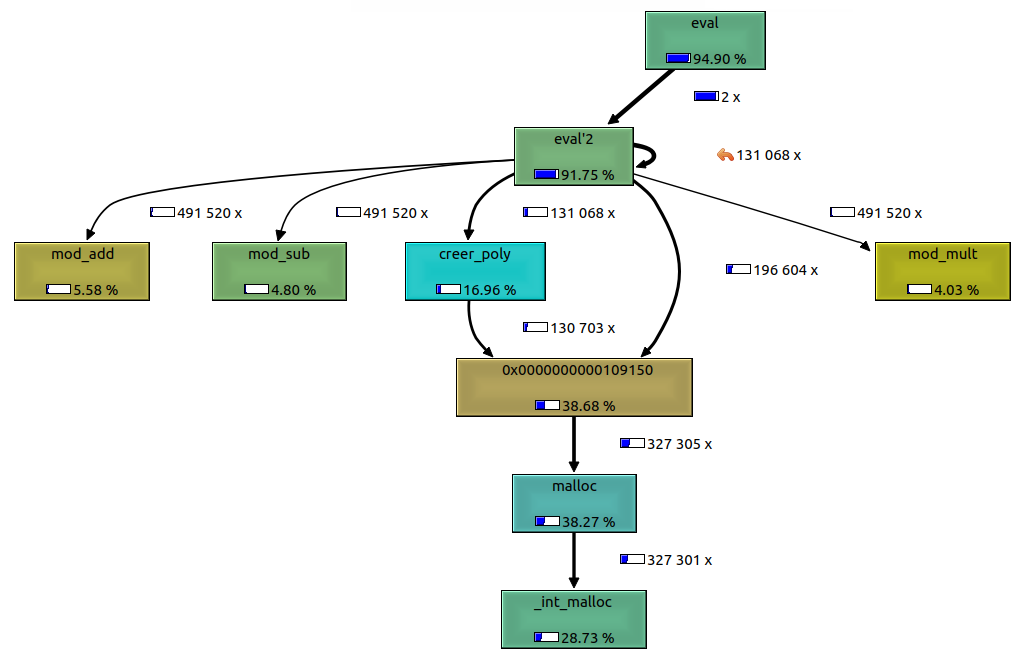
\includegraphics[scale=0.7]{profiler_eval_malloc}}

Constatant que les malloc représentent environ 40\% du temps d'exécution de notre fonction, notre priorité a été de réduire le nombre de malloc afin d'optimiser celle-ci.  \\
Nous avons d'abord remarqué que nous pouvions enlever le malloc pour le tableau $racines\_bis$. En effet, ce tableau sert à stocker les valeurs des cases $0,2,\dots,n$ du tableau $racines$, il était donc possible de se passer du tableau $racines\_bis$ en donnant en paramètre un pas $pas\_rac$ que nous multiplions par deux à chaque tour. \\
Concernant le malloc des tableaux de $R_0$ et $R_1$ de tailles $\frac{n}{2}$, nous avons pu les enlever en stockant les coefficients de $R_0$ dans la première moitié du tableau de $P$ (de taille n) et ceux de $R_1$ dans la seconde moitié. Ceci étant grâce au fait que nous n'ayons plus besoin de $P$ aux prochains tours de récursion.
Comme prévu la nouvelle fonction optimisée (fonction $eval()$) est plus rapide que la première version :

\begin{center}
\begin{tabular}{||c c c||}
\hline
Degré (+1) & $eval\_malloc()$ & $eval()$ \\
\hline\hline
$2^{21}$ & 0.769839 & 0.216310 \\
\hline
$2^{22}$ & 1.454626 & 0.561354 \\
\hline
$2^{23}$ & 2.825178 & 1.398087 \\
\hline
$2^{24}$ & 5.641160 & 3.615043 \\
\hline
\end{tabular}
\end{center}

\newpage

\section{Implémentation de la vectorisation dans la FFT avec AVX2}

Pour que notre FFT soit encore plus rapide, nous avons eu recours à la vectorisation avec AVX2. AVX2 nous permet de faire un certain nombre d'opérations (addition, soustraction...) beaucoup plus rapidement qu'avec les opérateurs de base du processeur que utilisons en C ($+$, $-$...). En effet, AVX2 permet de créer un type de variable ($\_\_m256i$) pouvant stocker 8 entiers de 32 bits (à l'image d'un tableau), ce qui convient parfaitement à la structure des polynômes. AVX2 pouvant réaliser une opération élémentaire sur deux $\_\_m256i$ aussi vite qu'une opération élémentaire sur deux $int$ en C, il est donc possible d'aller jusqu'à 8 fois plus vite avec AVX2. Voici un exemple de l'addition de deux $\_\_m256i$ en AVX2 : 

\begin{lstlisting}
__m256i a = _mm256_set_epi32(1, 2, 3, 4, 5, 6, 7, 8);
__m256i b = _mm256_set_epi32(1, 0, 1, 0, 1, 0, 1, 0);
__m256i x = _mm256_add_epi32(a, b);
// nous avons x == [2, 2, 4, 4, 6, 6, 8, 8]
\end{lstlisting}

\indent Voici un lien qui recense toutes les fonctions qu'offre AVX2 (les fonctions des  autres types SIMD / AVX / AVX512 etc. sont aussi disponibles) : \href{https://www.intel.com/content/www/us/en/docs/intrinsics-guide/index.html#techs=AVX,AVX2}{\underline{\color{blue}Site Intel}}

\subsection{Opération modulo p avec AVX2}

Pour des raisons de lisibilité nous allons illustrer cette partie avec des exemples de tableaux de taille 2. \\
\indent Le problème avec AVX2 est qu'il n'y a pas d'opération modulo, de plus, comme nous opérons directement sur 8 entiers en même temps, il est difficile de faire le modulo comme dans la partie 2.1.2.
Par exemple, pour l'addition supposons que : \\
\indent \indent $p = 7, \ \overrightarrow{a} = [6, 2], \ \space \overrightarrow{b} = [4, 1]$ \ et $ \ \overrightarrow{x} = \overrightarrow{a}+\overrightarrow{b}$ \\
Nous avons $\overrightarrow{x}[0] = 10$ et $\overrightarrow{x}[1] = 3$, nous devrions donc retirer $p$ pour faire le modulo sur $\overrightarrow{x}[0]$, mais alors nous aurions $\overrightarrow{x}[1] = 3-7 = -4$, ce qui n'est pas le résultat attendu.\\ 
\indent Pour faire l'addition et la soustraction modulo, il faut savoir qu'AVX2 nous permet de prendre les minimums "positif" sur chaque cases de deux $\_\_m256i$ (tous les nombres négatifs vont être converti en $Uint$), par exemple :\\ $min\_pos([1, 0],\  [0, -10]) = min([1, 0], \ [0,$ UINT\_MAX$-10]) = [0, 0]$ et non $[0, -10]$. \\
\indent Pour l'addition, avec $\overrightarrow{x} = \overrightarrow{a}+\overrightarrow{b}$, nous faisons l'opération $min\_pos(\overrightarrow{x},\ \overrightarrow{x}-\overrightarrow{p})$ où \overrightarrow{p} est un $\_\_m256i$ ne contenant que des $p$. Ceci permet bien de faire le modulo car si $\overrightarrow{a}[i] + \overrightarrow{b}[i] = \overrightarrow{x}[i] \geq p$, alors l'appel retourne $\overrightarrow{x}[i] - p$. Sinon, nous avons $\overrightarrow{a}[i] + \overrightarrow{b}[i] = \overrightarrow{x}[i] < p$, donc $\overrightarrow{x}[i]-p < 0$, et après conversion en $Uint$, $\overrightarrow{x}[i]-p$ sera plus grand que \overrightarrow{x}[i] et donc l'opération retournera \overrightarrow{x}[i]. Ceci correspond bien aux différents cas vus dans la partie 2.1.2. \\
C'est la même logique pour la soustraction $\overrightarrow{x} = \overrightarrow{a}-\overrightarrow{b}$, nous prenons $min\_pos(\overrightarrow{x},\ \overrightarrow{x}+\overrightarrow{p})$. \\
\indent Pour la multiplication, nous avons utilisé l'algorithme de réduction de Barrett, nous nous sommes inspirés de la source \cite{SIMD} qui montre comment faire cet algorithme avec vectorisation sur des entiers 16 bits.

\subsection{Comparaison de temps des opérations sans et avec AVX2}

Dans cette partie, nous allons comparer les temps d'exécution pour les opérations d'addition, de soustraction et de multiplication modulo p sans AVX et avec AVX. Pour cela, nous avons fait les opérations sur deux tableaux de taille 8 000 000.

\begin{center}
\begin{tabular}{||c c c||}
\hline
Opération & Sans AVX2 & Avec AVX2 \\
\hline\hline
Addition & 0.012610 & 0.006697 \\
\hline
Soustraction & 0.014247 & 0.007139 \\
\hline
Multiplication & 0.015053 & 0.007497 \\
\hline
\end{tabular}
\end{center}

Ici nous gagnons un facteur 2 grâce à AVX2 sur notre machine. Toutefois il est possible d'avoir un facteur plus grand selon la machine. En effet AVX2 provient de la marque Intel, il sera donc bien évidemment plus performant sur un processeur Intel. Il existe d'autres implémentations plus performantes que nous verrons plus tard (cf 3.4).  A VOIR

\subsection{Implémentation dans la DFT}

Nous voyons que dans l'algorithme de DFT, nous devons faire des opérations d'addition ($p_i+p_{i+k}$), de soustraction et de multiplication ($(p_i-p_{i+k})*\omega^i$). \\
L'implémentation de l'addition et de la soustraction vectorisée dans la DFT est plutôt directe, nous faisons une boucle dont l'indice augmente de 8 en 8 en passant les tableaux de taille 8 correspondants dans les fonctions de vectorisation. \\
\indent De plus, nous pouvons remarquer que l'addition et la soustraction se font avec les mêmes coefficients ($p_i$ et $p_{i+k}$). Nous voyons aussi que dans les fonctions $vect\_mod\_add()$ et $vect\_mod\_sub()$, nous devons charger les tableaux en $\_\_m256i$ à chaque fois (avec la fonction $\_mm256\_loadu\_si256()$). Pour optimiser, nous avons donc créé la fonction $vect\_mod\_add\_sub\_eval()$ qui permet de faire l'addition et la soustraction en ne chargeant qu'une fois les deux tableaux. \\[0.2cm]

\begin{customFrame}
void vect_mod_add_sub_eval(Uint *res_add, Uint *res_sub, Uint *tab1, Uint *tab2) {
    __m256i x, result; 
    // chargement du tableau avec que des p
    __m256i p = _mm256_set1_epi32(NB_P); 
    // chargement de 8 cases successives de tab1
    __m256i a = _mm256_loadu_si256((__m256i *) tab1); 
    // chargement de 8 cases successives de tab2
    __m256i b = _mm256_loadu_si256((__m256i *) tab2); 

    // addition modulo p
    // x = a + b
    x = _mm256_add_epi32(a, b); 
    // min_pos(x, x - p) (a+b)%p
    result = _mm256_min_epu32(x, _mm256_sub_epi32(x, p)); 
    // stockage du resultat dans res_add
    _mm256_storeu_si256((__m256i *) res_add, result);

    // soustraction modulo p
    // x = a - b
    x = _mm256_sub_epi32(a, b);
    // min_pos(x, x + p) = (a-b)%p
    result = _mm256_min_epu32(x, _mm256_add_epi32(x, p)); 
    // stockage du resultat dans res_sub
    _mm256_storeu_si256((__m256i *) res_sub, result);
}
\end{customFrame}
\ \\
\indent Désormais, pour la multiplication $(p_i-p_{i+k})*\omega^i$, le principal problème que nous avons rencontré est le pas $pas\_rac$ pour le tableau $racines$. En effet, nous voyons que dans la fonction sans AVX2 : $eval()$, dans la première boucle $for$, nous devons accéder à la case $i*pas\_rac$. Donc en travaillant sur des tableaux de taille 8 avec AVX2, il faudrait que nous accédions aux cases $(i+0)*pas\_rac,(i+1)*pas\_rac,\dots,(i+7)*pas\_rac$. 
Malheureusement notre fonction $\_mm256\_loadu\_si256()$ ne nous permet que de charger 8 cases à la suite (les cases $i+0, i+1,\dots,i+7$).
Cependant, nous avons trouvé la fonction $\_mm256\_i32gather\_epi32()$ qui prend en paramètre deux tableaux $\_\_m256i$ : $tab$ et $indices$ où $indices$ contient les indices des éléments que nous voulons avoir dans $tab$, la fonction prend aussi un entier $scale$ qui représente la taille en octet des éléments dans $tab$. Ce qui fait qu'ici, $tab$ correspond au tableau $racines$, $indices$ au tableau $[(i+0)*pas\_rac,\ (i+1)*pas\_rac,\ \dots,\ (i+7)*pas\_rac]$ et $scale$ à 4 (taille d'un $int$).\\
\indent Pour charger les cases voulues du tableau $racines$, il nous suffit alors de créer $indices$ grâce aux tableaux : \\ $\overrightarrow{i} = [i,\ \dots,\ i],\  \overrightarrow{u} = [0, 1, 2, 3, 4, 5, 6, 7]$ et $ \overrightarrow{pas} = [pas\_rac,\ \dots,\ pas\_rac]$. \\
Ce qui nous donne $indices = (\overrightarrow{i}+\overrightarrow{u})*\overrightarrow{pas}$. \\
Voici donc les temps obtenus après ces implémentations :

\begin{center}
\begin{tabular}{||c c c||}
\hline
Degré (+1) & Sans AVX2 & Avec AVX2 \\
\hline\hline
$2^{20}$ & 0.060076 & 0.056392 \\
\hline
$2^{21}$ & 0.175610 & 0.147659 \\
\hline
$2^{22}$ & 0.380583 & 0.333849 \\
\hline
$2^{23}$ & 0.975016 & 0.775812 \\
\hline
$2^{24}$ & 2.470365 & 2.090264 \\
\hline
\end{tabular}
\end{center}

\subsection{Multiplication des polynômes par FFT}
L'étape 2 de l'algorithme de multiplication de deux polynômes par FFT étant terminée, nous allons devoir implémenter les étapes 3 et 4 de cet algorithme. \\
Nous pouvons voir que l'étape 3 se résume en une boucle de $n$ multiplications. De plus, grâce à notre algorithme de multiplication modulo avec AVX2, nous pouvons vectoriser cet étape facilement. \\
Désormais, pour l'étape 4, nous avions vu dans la partie 2.1 qu'il suffisait essentiellement de réutiliser la DFT avec l'inverse des racines principales. En effet, pour faire cet étape nous devons calculer les puissances successives de l'inverse de la racine principale, appliquer la DFT à $Eval(R)$ sur ces inverses, et enfin, diviser les coefficients obtenus par la DFT par $n$ (c'est-à-dire multiplier par l'inverse de $n$ sur $\mathbb{Z}/p\mathbb{Z}$). \\
Nous avons donc créé un algorithme pour inverser un nombre sur le corps $\mathbb{Z}/p\mathbb{Z}$ en résolvant l'équation $a*u + b*v=1$ qui est en fait l'algorithme d'Euclide étendu. Dans notre cas nous avons $racine$ et $p$ premiers entre eux. Ainsi nous savons qu'il existe $u$ et $v$ tels que $racine*u + p*v=1$. De plus, comme nous sommes dans $\mathbb{Z}/p\mathbb{Z}$, tous les calculs se font avec un modulo $p$. Ainsi le calcul se simplifie en $racine*u\ \%\ p = 1$ et nous trouvons donc $u = racine^{-1}$ par définition de l'inverse. Grâce à cet algorithme, nous avons donc pu terminer l'étape 4. Par ailleurs, pour l'étape de division par $n$, cela consistait à la même chose que l'étape 3 de la FFT, nous avons donc pu la vectoriser aussi. Ceci conclut donc l'implémentation de la multiplication de polynômes par FFT. \\
Après avoir vérifié que notre multiplication par la FFT (avec ou sans AVX2) nous donnait des résultats correctes en les confrontant à ceux obtenus avec l'algorithme naïf, nous avons comparé les temps obtenus avec et sans AVX2.

\begin{center}
\begin{tabular}{||c c c||}
\hline
Degré (+1) & Sans AVX2 & Avec AVX2 \\
\hline\hline
$2^{20}$ & 0.158404 & 0.150727 \\
\hline
$2^{21}$ & 0.503089 & 0.437402 \\
\hline
$2^{22}$ & 1.240285 & 1.075995 \\
\hline
$2^{23}$ & 3.028623 & 2.317684 \\
\hline
$2^{24}$ & 7.108149 & 5.847869 \\
\hline
\end{tabular}
\end{center}

\subsection{Améliorations}

Pour finir, nous avons essayé de chercher des librairies faisant aussi la FFT (ou DFT suffit) vectorisée avec AVX2 sur $\mathbb{Z}/p\mathbb{Z}$ pour voir quelles sont les meilleures implémentations que nous pouvons avoir à ce jour. Nous sommes notamment tombé sur la librairie NTL (codée en C++) qui propose cela. Après installation de la librairie sur notre ordinateur, nous avons pu exécuter la DFT que propose NTL avec notre nombre premier $p = 754974721$ et avec $n = 2^{24}$. Nous avons tout d'abord exécuté leur DFT avec AVX2, cela donnait un temps d'environ XXXX, puis nous l'avons exécuté sans AVX2 pour un temps de XXXX. Nous voyons qu'il est possible de gagner un facteur au moins X grâce à AVX2, alors que dans notre implémentation nous n'avons même pas un facteur 2. \\
Nous avons donc fait quelques tests pour voir quelles opérations nous prenaient le plus de temps dans notre DFT et nous avons vu que c'était l'étape de multiplication qui prenait énormément de temps et plus spécifiquement lorsque nous voulons chercher dans le tableau $racines$ les cases voulues. Après réflexion, nous avons repensé à notre fonction $eval\_malloc()$ où nous faisons un $malloc$ à chaque tour pour créer le tableau $racines\_bis$ où toutes les racines que nous allons utiliser se suivent. Nous avons donc remis cette mécanique et n'avions donc plus besoin du pas $pas\_rac$ et donc utiliser la fonction de multiplication avec AVX2 sans avoir à chercher des indices spécifiques dans le tableau $racines$. Après tests, cela nous a fait gagner beaucoup de temps pour des degrés grands, les voici : 

\begin{center}
\begin{tabular}{||c c c||}
\hline
Degré (+1) & Sans AVX2 & Avec AVX2 (Version 2) \\
\hline\hline
$2^{20}$ & 0.158404 & 0.180472 \\
\hline
$2^{21}$ & 0.503089 & 0.355293 \\
\hline
$2^{22}$ & 1.240285 & 0.706925 \\
\hline
$2^{23}$ & 3.028623 & 1.504402 \\
\hline
$2^{24}$ & 7.108149 & 2.939824 \\
\hline
\end{tabular}
\end{center}

Nous voyons que cette fois-ci nous avions plus d'un facteur 2 pour de gros degré.

\section{Temps}

\begin{center}
\begin{tabular}{||c c c||}
\hline
Degré (+1) & Sans AVX2 & Avec AVX2 \\
\hline\hline
$2^{20}$ & 0.190341 & 0.141107 \\
\hline
$2^{21}$ & 0.400805 & 0.290091 \\
\hline
$2^{22}$ & 0.831379 & 0.613087 \\
\hline
$2^{23}$ & 1.789433 & 1.346448 \\
\hline
$2^{24}$ & 6.257555 & 4.494047 \\
\hline
\end{tabular}
\end{center}

\newpage

\bibliographystyle{plain}
\bibliography{biblio}

\end{document}
